\section{Conflict-serializability}

\begin{definition}
    Two operations $o_i$ and $o_j$ ($i \neq j$) are in \emph{conflict} if they address the same resource and at least one of them is write. There are two possible cases:
    \begin{enumerate}
        \item Read-write conflicts ($r-w$ or $w-r$).
        \item Write-write conflicts ($w-w$).
    \end{enumerate}

    Two schedules are \emph{conflict-equivalent} ($S_i \approx_C S_j$) if $S_i$ and $S_j$ contain the same operations and in all the conflicting pairs the transactions occur 
    in the same order. 

    A schedule is \emph{conflict-serializable} (CSR) if and only if it is conflict equivalent to a serial schedule of the same transactions. 
\end{definition}
We have that VSR is a strict subset of CSR and that CSR implies VSR. 
\begin{proof}[VSR is a subset of CSR]
    Schedule $S = r_1(x) w_2(x) w_1(x) w_3(x)$ is: 
    \begin{itemize}
        \item View-serializable.
        \item Not conflict-serializable
    \end{itemize}
    It is possible to check that there is no conflict-equivalent serial schedule.
\end{proof}
\begin{proof}[CSR implies VSR]
    We assume $S_1 \approx_C S_2$ and prove that $S_1 \approx_V S_2$. $S_1$ and $S_2$ must have: 
    \begin{itemize}
        \item The same final writes: if they didn't, there would be at least two writes in a different order, and since two
            writes are conflicting operations, the schedules would not be $\approx_C$. 
        \item The same reads-from relations: if not, there would be at least one pair of conflicting operations in a different
            order, and therefore, again, $\approx_C$ would be violated. 
    \end{itemize}
\end{proof}
The testing of view-serializability is done with a conflict graph that has one node for each transaction $T_i$, and one arc from $T_i$ to $T_j$ if there exists at least one conflict between an operation $o_i$ of $T_i$ and an operation $o_j$ of $T_j$ such that $o_i$ precedes $o_j$.
\begin{theorem}
    A schedule is \emph{conflict-serializable} if and only if its conflict graph is acyclic.
\end{theorem}
\begin{example}
    We are given the schedule \[S: w_0(x) r_1(x) w_0(z) r_1(z) r_2(x) w_0(y) r_3(z) w_3(z) w_2(y) w_1(x) w_3(y)\]
    To test the conflict serializability we have to do the following steps: 
    \begin{enumerate}
        \item Create all the nodes based on the number of transactions of the schedule. 
        \item Divide the operation based on resource requested.
        \item Check all the write-write and read-write relationships in each subset, and add the arcs based on these. 
    \end{enumerate}
    In the given example we obtain: 
    \begin{itemize}
        \item $x: w_0 r_1 r_2 w_1$
        \item $y: w_0 w_2 w_3$
        \item $z: w_0 r_1 r_3 w_3$
    \end{itemize}
    \begin{figure}[H]
        \centering
        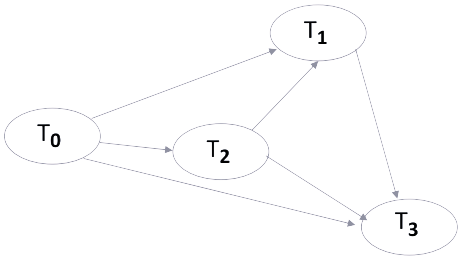
\includegraphics[width=0.5\linewidth]{images/conflict.png}
    \end{figure}
    There are no cycles in the graph, so this means that the schedule is CSR. 
\end{example}
\begin{proof}[CSR implies acyclicity of the conflict graph]
    Consider a schedule $S$ in $CSR$. As such, it is $\approx_C$ to a serial schedule. 
    Without loss of generality we can label the transactions of $S$ to say that their order in the serial schedule is: $T_1 T_2 \dots T_n$.
    Since the serial schedule has all conflicting pairs in the same order as schedule $S$, in the conflict graph there can only be arcs $(i,j)$, with $i<j$. 
    Then the graph is acyclic, as a cycle requires at least an arc $(i,j)$ with $i>j$.
\end{proof}
\begin{proof}[acyclicity of the conflict graph implies CSR]
    If $S$'s graph is acyclic then it induces a topological (partial) ordering on its nodes. The same partial order exists on the transactions of $S$. 
    Any serial schedule whose transactions are ordered according to the partial order is conflict-equivalent to $S$, because for all conflicting pairs $(i,j)$ it is always $i<j$. 
\end{proof}